\documentclass[a4paper,10pt]{book}

\usepackage[latin1]{inputenc}
\usepackage[italian]{babel}
\usepackage[pdftex]{graphicx}

\title{Machine Learning e Reti Neurali}
\author{Davide Gessa}
\date{25 Aprile 2010}

\pdfinfo{
  /Title    (Reti neurali)
  /Author   (Davide Gessa)
  /Subject  ()
  /Keywords (reti neurali fuzzy statistica matematica)
}

\begin{document}
\maketitle

\tableofcontents
\setcounter{tocdepth}{4}
\listoffigures
\listoftables


\chapter{Introduzione}
Questa tesi nasce da un vecchio software da me iniziato verso l'inizio del 2009 (e
mai terminato) che riassumeva il frutto di qualche mia curiosita' riguardo 
l'argomento delle reti neurali artificiali; qualche mese fa ho ritrovato i sorgenti 
e mi sono 
reinteressato all'argomento, riscrivendo da zero un nuovo software (che analizzero' 
in seguito) che implementa alcuni tipi di reti neurali artificiali e alcune
loro applicazioni
pratiche. Avevo gia' iniziato una breve trattazione da esporre su un altro mio
progetto, ma ho deciso di iniziare da capo per dedicarmi ad un argomento che
raccoglie in se' piu' materie, come statistica, matematica, informatica e per certe
caratteristiche tecniche del mio progetto anche sistemi.
Per vedere lo sviluppo dei miei progetti "inventati.org/dak".

\section{Licenza}
Il proggetto e' rilasciato interamente sotto licenza GPLv2, presente integralmente
nel file "license.txt"; e' riportato qui di 
seguito l'header presente in ogni file sorgente del progetto:
\newline
\newline 
\ttfamily
\textit
    libneuralnetwork
    Copyright (C) 2010 Davide Gessa
    
    This program is free software: you can redistribute it and/or modify
    it under the terms of the GNU General Public License as published by
    the Free Software Foundation, either version 2 of the License, or
    (at your option) any later version.

    This program is distributed in the hope that it will be useful,
    but WITHOUT ANY WARRANTY; without even the implied warranty of
    MERCHANTABILITY or FITNESS FOR A PARTICULAR PURPOSE.  See the
    GNU General Public License for more details.

    You should have received a copy of the GNU General Public License
    along with this program.  If not, see <http://www.gnu.org/licenses/>.
\rmfamily
\newline


\section{Strumenti software}
Ecco una lista dei software principali utilizzati per realizzare il progetto e la tesi
che state leggendo; da sottolineare che tutti sono free software e opensource, e che 
lo sviluppo e' avvenuto col sistema operativo gnu/linux gentoo per lo sviluppo ed i test, 
anch'esso free e opensource.

\begin{description}
\item[gcc] compilatore per il linguaggio C
\item[cmake] sistema di compilazione
\item[geany] C and \LaTeX ide
\item[subversion] controllo di revisione
\item[gtk+] librerie per interfacce grafiche
\item[gnuplot] programma di plotting matematico
\item[latex] compilatore per il linguaggio \LaTeX
\end{description}



\section{\LaTeX}
Per scrivere la documentazione del sistema e' stato utilizzato il linguaggio di markup
\LaTeX, che permette di preparare dei testi basati su \TeX, un linguaggio di composizione 
tipografica. Utilizzare \LaTeX, permette di risparmiare un tempo notevole per quanto riguarda
la formattazione delle pagine, la creazione degli indici, la visualizzazione di formule matematiche
e molto altro, e per questo motivo e' utilizzato da gran parte di accademici, scienziati, matematici
e ingegneri. \LaTeX e' distribuito come software libero ed e' disponibile su molte piattaforme.





\chapter{Reti neurali}
Questo progetto mira ad esporre il funzionamento di una rete neurale artificiale
e di alcuni algoritmi per l'apprendimento; e' comunque necessario fare una breve
introduzione riguardo il funzionamento delle reti neurali in natura.

\section{Reti neurali biologiche}
Il funzionamento delle reti neurali artificiali, deriva da degli studi effetuati
sulle reti neurali biologiche, presenti ad esempio nel cervello degli animali; 
i primi successi significativi riguardo lo studio 
del funzionamento delle reti neurali sono relativamente recenti, e alcuni aspetti
del loro funzionamento sono ancora ignoti.
Le reti neurali sono delle strutture costituite da neuroni; 
I neuroni sono classificabili secondo diverse caratteristiche, una di queste
e' la loro funzione:
\begin{itemize}
\item Neuroni sensitivi o neuroni di input: si occupano di ricevere impulsi e stimoli 
		dagli organi sensoriali.
\item Neuroni motori o neuroni di output: generano impulsi di tipo motori che vengono
		trasmessi agli organi periferici.
\item Interneuroni o neuroni nascosti: elaborano le informazioni fornite dai neuroni 
		sensitivi per trasmetterle ai neuroni motori.
\end{itemize}

Ogni neurone (che sia sensitivo, motorio o un interneurone) e' formato 
principalmente da tre parti:
\begin{itemize}
\item La soma: che comprende il corpo cellulare compreso il nucleo e altri apparati 
		dedicati alla sopravvivenza della cellula.
 
\item Gli assoni: conducono il segnale generato dal soma verso altre cellule neurali.
 
\item I dentriti: son costituiti da diramazioni ad albero che trasportano segnali di 
		altri neuroni, verso la soma; i dentriti hanno la caratteristica di non essere 
		buoni
		conduttori di segnali nervosi, i segnali ricevuti tendono quindi a diminuire di
		intensita'.
%capire bene assone e dentriti
\end{itemize}


% Immagine da cambiare urgentemente
\begin{figure}[h]
	\begin{center}	
		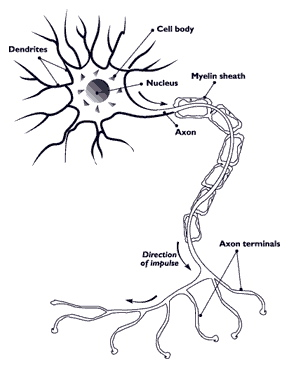
\includegraphics[scale=0.50]{img/neuron.jpg}
		\caption{Struttura di un neurone}
		\label{fig: Struttura di un neurone}
	\end{center}
\end{figure}
 
\subsection{Trasmissione delle informazioni tra neuroni}
Gli assoni e i dentriti, comunicano con altre cellule neurali
attraverso dei punti di connessione detti sinapsi. La trasmissione
di un informazione da un neurone all'altro avviene attraverso
l'emmissione  di sostanze chimiche dette neuro-trasmettitori 
stimolata da segnali chimici o da segnali elettrici 
generati dal neurone stesso.

% Parla delle sinapsi, delle connessioni e dei pesi



\section{Reti neurali artificiali}
Le reti neurali artificiali sono in sostanza, dei modelli matematici composti
da neuroni artificiali o nodi (strutture matematiche che hanno il compito
di emulare in parte il funzionamento di un neurone biologico) e dalle loro 
interconnessioni che simulano il funzionamento di una rete neurale biologica;
le reti neurali artificiali permettono di risolvere problemi quindi
di intelligenza artificiale, a seguito di un periodo nel quale la rete verra'
istruita a svolgere dei compiti (fase di apprendimento).

%parla dei problemi di regressione

\subsection{Storia}

\subsection{Tipi di rete}
Parlare delle reti feedfoward

\subsubsection{Multi Layered Perceptons}
\subsubsection{Self Organization Map}
\subsubsection{Hopefield}

\subsection{Apprendimento}
Per poter utilizzare la rete per scopi pratici, bisogna prima addestrarla
opportunamente per trovare (piu' precisamente imparare) la relazione
tra dati di input e dati di output. L'addestramento puo' essere
eseguito con svariati tipi di algoritmo, ma fondamentalmente si
possono distinguere tre metodi di apprendimento:

\begin{itemize}
\item Supervisionato: consiste nel proporre alla rete dei set di dati di input e i 
corrispettivi
dati di output (risultato degli input); tramite un algoritmo, la rete
impara il legame che c'e' tra essi.
Uno degli algoritmi chiave dell'apprendimento supervisionato, e' l'algoritmo
di propagazione inversa (meglio noto come backpropagation), che mediante
un pattern di input ed uno di output, calcola l'errore per ogni strato
della rete ricalcolando i pesi sinaptici dei singoli neuroni.
L'algoritmo di backpropagation verra' analizzato nei dettagli
nell'articolo dedicato alle reti MLP.

\item Non supervisionato: non prevede nessun intervento esterno, bensi' utilizza
metodi probabilistici per individuare dei possibili input e dei corrispondenti
risultati di output.
%introduci l'algoritmo senza supervisione delle reti SOM

\item Per rinforzo: un algoritmo si occupa di generare azioni e di interpetare il risultato della
retroazione dell'ambiente stesso, valutando se tale retroazione e' positiva
o negativa per raggiungere lo scopo prefissato dalla rete.
% verificare
\end{itemize}



\chapter{Reti MLP e apprendimento supervisionato}
Le reti neurali mlp sono

\section{Elenco dei simboli}
\begin{table}[h]
	\begin{center}
	    \begin{tabular}{  c  c  }
	    $ \delta_i $ & Errore del neurone i \\ 
	    $ \eta $ & Costante di apprendimento \\ 
	    $ \omega_i^k $ & Peso sinaptico del neurone i rispetto al neurone k \\
	    $ x_i $ & Valore del neurone di input i \\ 
	    $ y_i $ & Valore del neurone hidden i \\ 
	    $ z_i $ & Valore del neurone di output i \\ 
	    \end{tabular}
	\end{center}
	\caption{Elenco dei simboli per le reti MLP}
	\label{tab:mlp_symbols}
\end{table}


\section{Back Propagation}
Il "back propagation" (propagazione inversa) e' un algoritmo di apprendimento
utilizzato nelle reti neurali feedfoward. 

1.
Per prima cosa si calcola l'errore delta dello strato di output; per ogni neurone dello 
strato di output si calcola la differenza tra il valore desiderato e quello
ottenuto dalla rete, poi il valore ottenuto viene moltiplicato per la derivata
della funzione di trasfermento, e come argomento della funzione il valore di
output ottenuto dalla rete cosi' come e' ora:

\[
 \delta_i = (desidered_i - output_i) * f'(output_i)
\]


2.
Ora calcoliamo l'errore delta di ognuno degli strati nascosti
della rete:

\[
 \delta_i = (\sum_{k=0}^{outputn}\delta_k * \omega_k) * f'(output_i)
\]



3.
Aggiorniamo ora i pesi sinaptici dei vari strati partendo da quello di 
output; per ogni neurone di output quindi:
\[
 \omega_i = (\sum_{k=0}^{hidden} \eta * hidden_k * \delta_output)
 %\sum_{k=0}^{outputn}\delta_k * \omega_k) * f'(output_i)
\]


%	// Aggiorna i pesi dello strato di output
%	for(j = 0; j < n->output_n; j++)
%	{
%		for(k = 0; k < n->hidden_n; k++)
%			(n->output[j]).weights[k] += n->learning_rate * (n->output[j]).delta * (n->hidden[k]).value;
%		(n->output[j]).bias += n->learning_rate * (n->output[j]).delta;
%	}

4.
Aggiorniamo i pesi degli strati nascosti:	

\[
 \omega_i = (\sum_{k=0}^{hidden} \eta * hidden_k * \delta_output)
 %\sum_{k=0}^{outputn}\delta_k * \omega_k) * f'(output_i)
\]

%	// Aggiorna i pesi dello strato hidden
%	for(j = 0; j < n->hidden_n; j++)
%	{
%		for(k = 0; k < n->input_n; k++)
%			(n->hidden[j]).weights[k] += n->learning_rate * (n->hidden[j]).delta * (n->input[k]).value;
%		(n->hidden[j]).bias += n->learning_rate * (n->hidden[j]).delta;
%	}



\section{Pattern Recognition mediante rete neurali}
Il pattern recognition (riconoscimento di pattern, in italiano), 
e' una delle possibili applicazioni delle reti neurali; 
il pattern recognition in se', e' un processo di 
riconoscimento e classificazione di pattern, partendo
da un insieme di dati grezzi in input.

\subsection{Applicazioni software}
Ho realizzato un piccolo programma in gtk+ per il riconoscimento
di pattern, fondamentalmente di lettere e numeri, ma con qualche
piccola modifica e' possibile utilizzarlo per altri tipi di dati.
Il programma permette di indicare una cartella contenente file png
(per ora solo 64x64 in scala di grigi), selezionare il numero di epoche, 
e avviare il processo di apprendimento; e' possibile poi utilizzare un altra 
immagine, con le stesse caratteristiche dei pattern di addestramento, 
per testare la rete ed ottenere in output la lettera corrispondente all'immagine. 


Ho realizzato vari set di pattern per fare dei test, in figura possiamo
vedere un test con le lettere cirilliche (translitterate in lettere latine).
\begin{figure}[h]
	\begin{center}	
		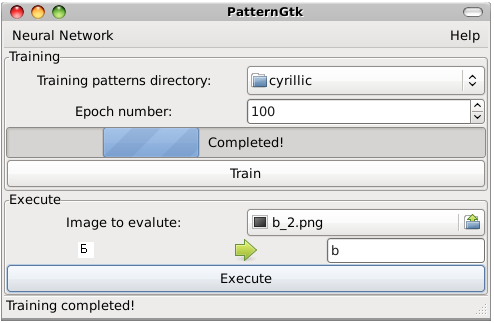
\includegraphics{img/screen/patrec1.png}
		\caption{Pattern Recognition in GTK+}
		\label{fig: Programma di Pattern Recognition in GTK+}
	\end{center}
\end{figure}


% Eseguendo per tutte le diverse n epoche prese in considerazione, l'operazione
%  di backpropagation (per n epoche) e l'esecuzione
% Test immagini
% Immagine con numero di epoche (x) probabilita' che il risultato sia corretto (100 test per ogni numero di epoche)
% Immagine tempo di 1 backpropagate (x) neuroni input + neuroni hidden + neuroni output (y) 


\chapter{Reti SOM e apprendimento senza supervisione}
Le reti SOM sono un particolare tipo di rete neurale feed-foward, 

\section{Apprendimento auto-organizzato}


%applicazione per visualizzarle con sdl

\chapter{Bibliografia}
\begin{thebibliography}{Bibliografia}
	\bibitem{lamport-latex2} Silvio Cammarata - Reti neurali, dal Percepton alle reti caotiche e neuro-fuzzy
	\bibitem{lamport-latex2} Christopher M. Bishop - Pattern Recognition and Machine Learning
\end{thebibliography}

\appendix


\end{document}

